% Compile with XeLaTeX, TeXLive 2013 or more recent
\documentclass{beamer}

% Base packages
\usepackage{fontspec}
\usepackage{xunicode}
\usepackage{xltxtra}

\usepackage{amsfonts}
\usepackage{amsmath}
\usepackage{longtable}
\usepackage{csquotes}
\usepackage{standalone}

% Setup fonts
\newfontfamily\russianfont{CMU Serif}
\setromanfont{CMU Serif}
\setsansfont{CMU Sans Serif}
\setmonofont{CMU Typewriter Text}

% Setup Russian hyphenation. NOTE: this declaration *must* come after fontspec's font declarations,
% or a mysterious (but harmless in other respects) error "Improper `at' size (0.0pt), replaced by 10pt." would appear.
\usepackage{polyglossia}
\defaultfontfeatures{Scale=MatchLowercase, Mapping=tex-text}

\setdefaultlanguage[spelling=modern]{russian} % for polyglossia
\setotherlanguage{english} % for polyglossia

% Vector drawings 
\usepackage{tikz}
\usetikzlibrary{shapes, calc, arrows, fit, positioning, decorations, patterns, decorations.pathreplacing, chains, snakes}

% Be able to insert hyperlinks
\usepackage{hyperref}
\hypersetup{colorlinks=true, linkcolor=black, filecolor=black, citecolor=black, urlcolor=blue , pdfauthor=Grigory Rechistov <grigory.rechistov@phystech.edu>, pdftitle=Моделирование OpenRISC 1000 на Wind River Simics}
% \usepackage{url}

% Misc optional packages
\usepackage{underscore}
\usepackage{amsthm}

\usepackage{ulem} % for strikethrough
\usepackage{bytefield} % for bitefield

% A new command to mark not done places
\newcommand{\todo}[1][Напиши меня]{{\color{red}TODO\ #1}}


\title{Моделирование OpenRISC 1000 (ч. 2)}
% \subtitle{Курс «Программное моделирование вычислительных систем»}
\subject{Лекция}
\author[Григорий Речистов]{Григорий Речистов \\ \small{\href{mailto:grigory.rechistov@intel.com}{grigory.rechistov@intel.com}}}
\date{26-28 августа 2014 г.}
\pgfdeclareimage[height=0.5cm]{intel-logo}{../images/intel.png}
\logo{\pgfuseimage{intel-logo}}

\typeout{Copyright 2014 Grigory Rechistov}

\usetheme{Berlin}
\setbeamertemplate{navigation symbols}{}%remove navigation symbols

\begin{document}

\begin{frame}
\titlepage
\end{frame}

\begin{frame}
\tableofcontents
\end{frame} 

\section{Повторение}

\begin{frame}{Вопросы}
\pause
\begin{itemize}
	\item Что такое модуль в Simics? \pause
	\item Что такое класс в Simics? \pause
	\item Что такое атрибут Simics?\pause
	\item Какие типы атрибутов бывают?\pause
	\item Что такое интерфейс Simics?

\end{itemize}

\end{frame}

\section{Отдельные инструкции}

\begin{frame}{Декодирование и дизассемблирование}

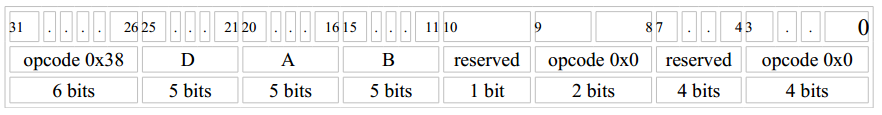
\includegraphics[width=\textwidth]{openrisc-format}

Делаем l.add

\end{frame}

\begin{frame}{Семантика}

\texttt{modules/or1k/or1k.c}

Функция \texttt{or1k_execute()}

\end{frame}


\begin{frame}{Тестирование}

\texttt{test/or1k/unit-tests/}

Пример \texttt{nop}:

\begin{itemize}
\item Подготавливаем данные и код.
\item Исполняем инструкцию.
\item Проверяем результаты.
\end{itemize}

\end{frame}

\begin{frame}{Повторяем!}
l.msync, l.bf, l.div, l.extbs, l.j, l.ld, l.ff1, l.jalr, l.macu, l.mul, l.ror, l.sb, l.sfgtsi, l.xori, l.sys

\end{frame}

\section{Литература}

\begin{frame}[allowframebreaks]{Литература}
\begin{thebibliography}{99}
	\bibitem{or1k-isa-spec}  Open Cores OpenRISC 1000 Architecture Manual. Architecture Version 1.0 Document Revision 0. — 2012. — URL: \url{http://opencores.org/websvn,filedetails?repname=openrisc&path=/openrisc/trunk/docs/openrisc-arch-1.0-rev0.pdf}
	\bibitem{model-builder} Simics Model Builder User Guide 4.6 / Wind River. — 2014.
	
\end{thebibliography}
\end{frame}


\section{Конец}
% The final "thank you" frame 
\begin{frame}

{\huge{Спасибо за внимание!}\par}

\vfill

Слайды и материалы курса доступны по адресу \url{http://bit.ly/1y1lZF1} % http://atakua.doesntexist.org/wordpress/tag/or1k/

\vfill

\tiny{\textit{Замечание}: все торговые марки и логотипы, использованные в данном материале, являются собственностью их владельцев. Представленная точка зрения отражает личное мнение автора.
%Материалы доступны по лицензии Creative Commons Attribution-ShareAlike (Атрибуция — С сохранением условий) 4.0 весь мир (в т.ч. Россия и др.). Чтобы ознакомиться с экземпляром этой лицензии, посетите \url{http://creativecommons.org/licenses/by-sa/4.0/}
}

\end{frame}

% \section{Резерв}

\end{document}
